\documentclass[11pt,letterpaper]{article}
\usepackage{amssymb,amsfonts,color,graphicx,amsmath,enumerate}
\usepackage{tikz}
\usepackage{amsthm}

\newcommand{\naturals}{\mathbb{N}}
\newcommand{\integers}{\mathbb{Z}}
\newcommand{\complex}{\mathbb{C}}
\newcommand{\reals}{\mathbb{R}}
\newcommand{\mcal}[1]{\mathcal{#1}}
\newcommand{\rationals}{\mathbb{Q}}
\newcommand{\Lp}[2]{\left\|{#1}\right\|_{L^{#2}}}
\newcommand{\field}{\mathbb{F}}
\newcommand{\affine}{\mathbb{A}}
\newcommand{\E}{\mathbb{E}}
\newcommand{\Prob}{\mathbb{P}}
\newcommand{\Var}{\text{Var}}
\newcommand{\ind}{\mathbbm{1}}
\newcommand{\Cov}{\text{Cov}}

\newenvironment{solution}
{\begin{proof}[Solution]}
{\end{proof}}

\voffset=-3cm
\hoffset=-2.25cm
\textheight=24cm
\textwidth=17.25cm
\addtolength{\jot}{8pt}
\linespread{1.3}

\begin{document}
\begin{center}
{\bf \Large Math 130B - Conditional Expectation and Moment Generating Functions}
\vspace{0.2cm}
\hrule
\end{center}

\begin{enumerate}
	\item A mouse is placed in a maze with two rooms pictured in Figure 1. Starting from room 1, what is the expected number of steps the mouse takes before it reaches the exit?
	\begin{figure}[h]
		\centering
		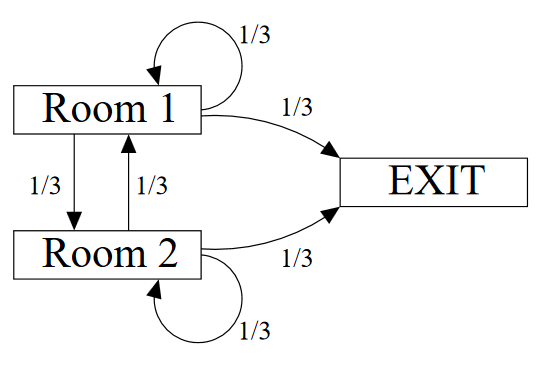
\includegraphics[scale=.7]{diagram.PNG}
		\caption{Mouse's actions}
	\end{figure}
	%30, 177

	\vfill

	\item You run a whale-watching business in San Diego.
	Every day you are unable to operate your tour due to bad weather with probability $p$, independently of all other days.
	You work every day except the bad-weather days.

	Let $Y$ be the number of consecutive days you work between bad-weather days and let $X$ be the total number of customers who attend your tour in this period of $Y$ days.
	Conditional on $Y$, suppose the distribution of $X$ is
	\[
		X\mid Y \sim \text{Pois}(\mu Y).
	\]
	\begin{enumerate}
		\item What kind of random variable is $Y$. What are its expectation and variance?
		\vfill

		\item Find the expectation and variance of the number of customers you see between bad weather days.
	\end{enumerate}

	\vfill\pagebreak

	\item A factory has produced $n$ robots, each of which is faulty with probability $\phi$. Each robot is tested to determine whether or not it is faulty. If the robot it faulty, the test detects the fault with probability $\delta$. Let $X$ be the number of faulty robots, and let $Y$ be the number detected as faulty. Under normal assumptions about dependence, show that
	\[
		\E[X\mid Y] = \frac{n\phi(1-\delta) + (1-\phi)Y}{1-\phi\delta}.
	\]
	\vfill

	\item Suppose that a statistician determines that the revenue the biological sciences Starbucks makes in a week is a random variable, $X$, with moment generating function
	\[
		m_X(t) = \frac{1}{(1-2500t)^4}.
	\]
	Find the standard deviation of the revenue the Starbucks makes in a week.

	\vfill

	\item Let $X$ and $Y$ be two independent random variables with respective moment generating functions
	\[
		m_X(t) = \frac{1}{1-5t},\ \text{if }t<1/5,\quad m_Y(t) = \frac{1}{(1-5t)^2},\ \text{if }t<1/5.
	\]
	Find $\E[(X+Y)^2]$.

	\vfill

	\item True or False? If $X$ and $Y$ are independent exponential random variables with parameters $\lambda_x$ and $\lambda_y$, respectively, then $X+Y$ is an exponential random variable with parameter $\lambda_x + \lambda_y$.
	\vfill
\end{enumerate}


\end{document}